\documentclass{beamer}
\usepackage{xeCJK}
\usepackage{listings}
\usepackage{graphicx}

\title{数据结构第一讲}
\subtitle{树状数组、线段树及ST表}
\author{丁尧尧}
\institute{上海交通大学}
\date{\today}
\usetheme{PaloAlto}

\begin{document}
	\maketitle
	\begin{frame}{目录}
		\tableofcontents
	\end{frame}
	
	\section{树状数组}
		\subsection{介绍}
			\begin{frame}{树状数组能做什么}
				我们知道,对于如下问题: \\
				\begin{block}{单点修改,区间求和} 
					给定$n$个数,要求支持:\\
					\begin{enumerate}
						\item 单点修改 modify u x
						\item 区间求和 query l r
					\end{enumerate}
				\end{block}
				我们一般有两种处理方式\\
				一种是用$a[i]$存储位置$i$的值,可以实现$O(1)$修改,$O(n)$查询。\\
				一种是用$s[i]$存储前$i$个数的和,可以实现$O(n)$修改,$O(1)$查询。\\
				但树状数组可以实现在完全相同的空间消耗上,完成$O(log(n))$的修改和查询。
			\end{frame}
		\subsection{实现}
			\begin{frame}[fragile=singleslide]
				\frametitle{我们先直接看看代码具体怎么实现的}
				\begin{verbatim}
void modify( int u, int x ) {
    for( int i = u; i <= n; i += lowbit(i) )
        a[i] += x;
}
void query( int r ) {
    int rt = 0;
    for( int i = r; i; i -= lowbit(i) )
        rt += a[i];
    return rt;
}
int query( int l, int r ) {
    return query(r) - query(l-1);
}
				\end{verbatim}
				其中\verb|lowbit(i)|返回i的最低位代表的数,可以通过\verb|(i & -i)|计算得到(采用补码的机子上)。
			\end{frame}
		\subsection{正确性和复杂度分析}
			\begin{frame}{正确性和复杂度分析}
				复杂度很显然都是$O(log(n))$,下面我们来看看为什么这么做是对的。
				\begin{definition}
					对于一个在$[1,n]$之间的整数$i$,我们通过
					不断给它加它的lowbit(直到它的值大于n)得到一个\textbf{递增序列},
					不断给它减它的lowbit(直到它的值变为0)得到一个\textbf{递减序列}。
				\end{definition}
				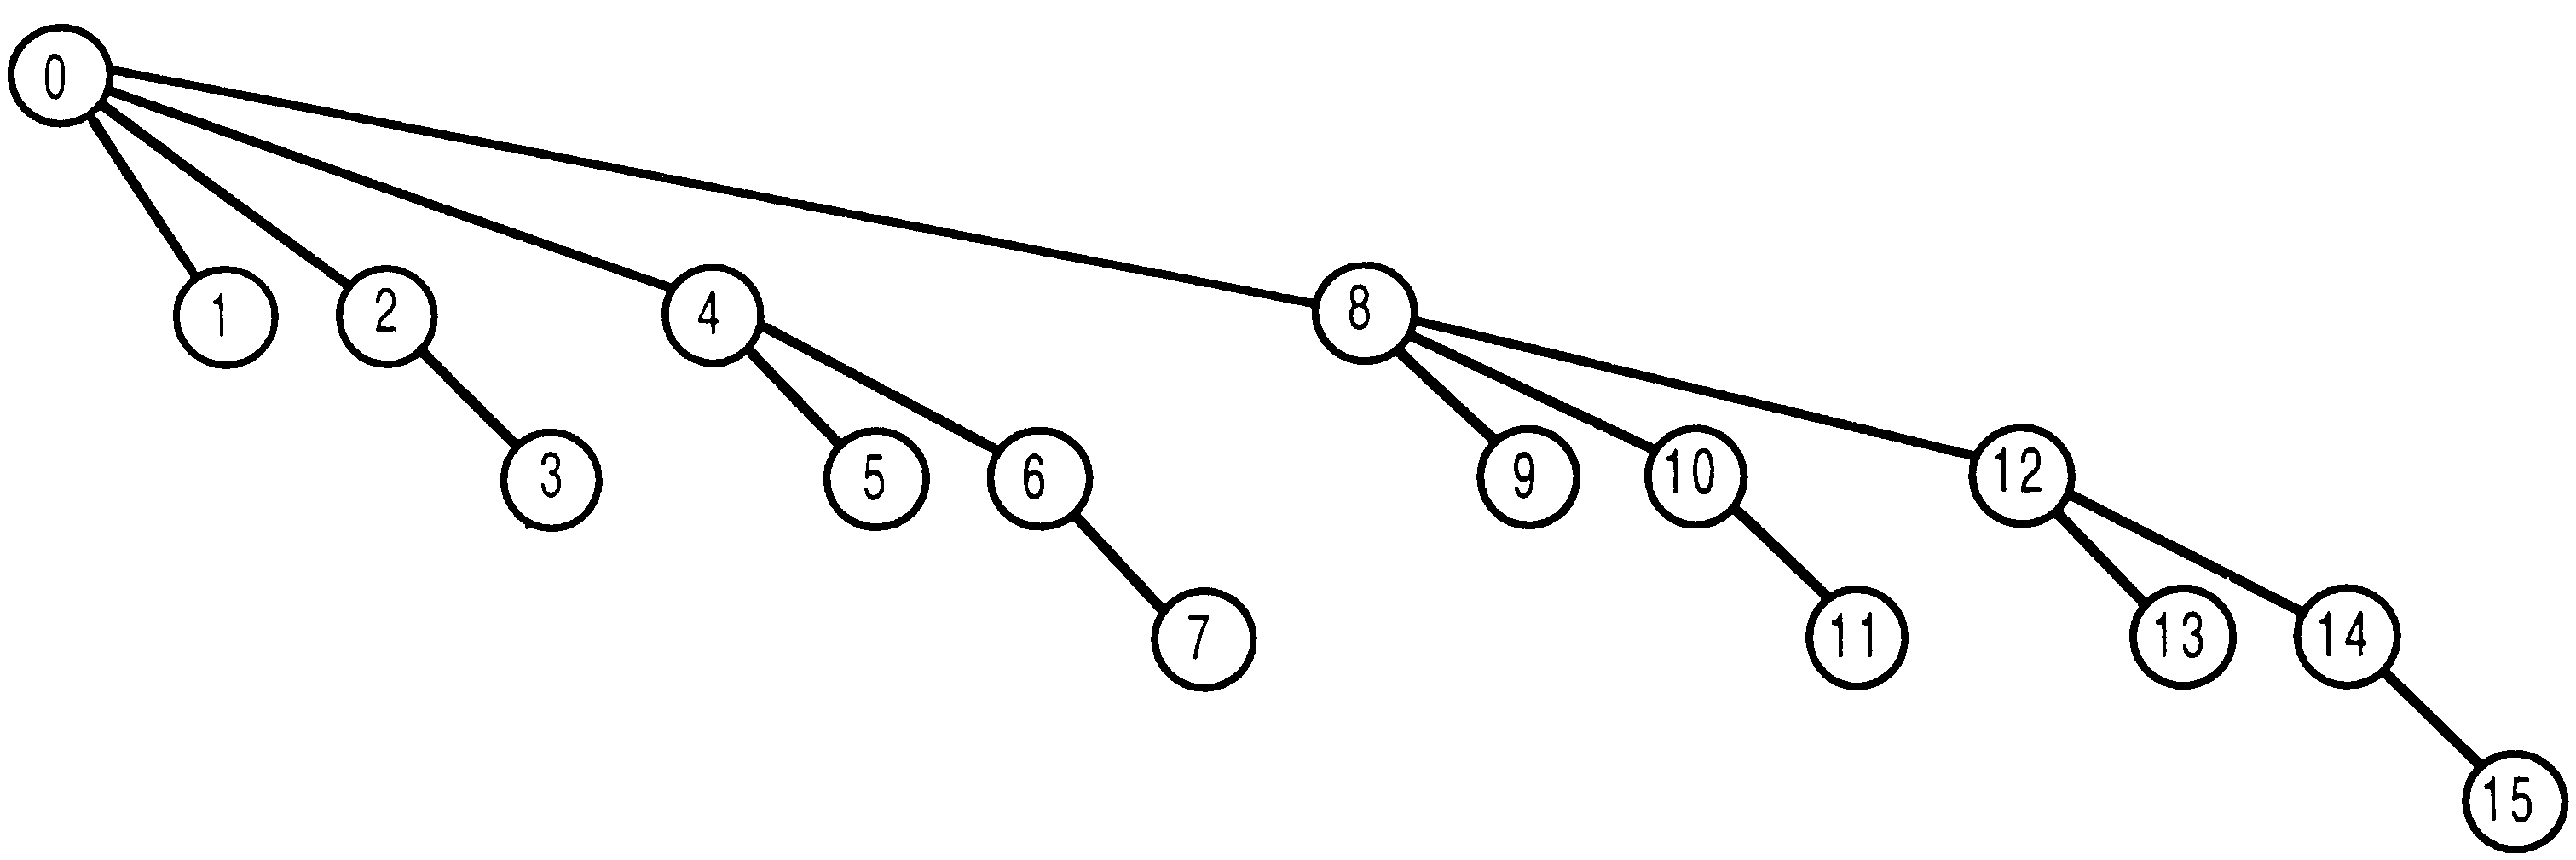
\includegraphics[height=1.7cm]{downseq.png}
				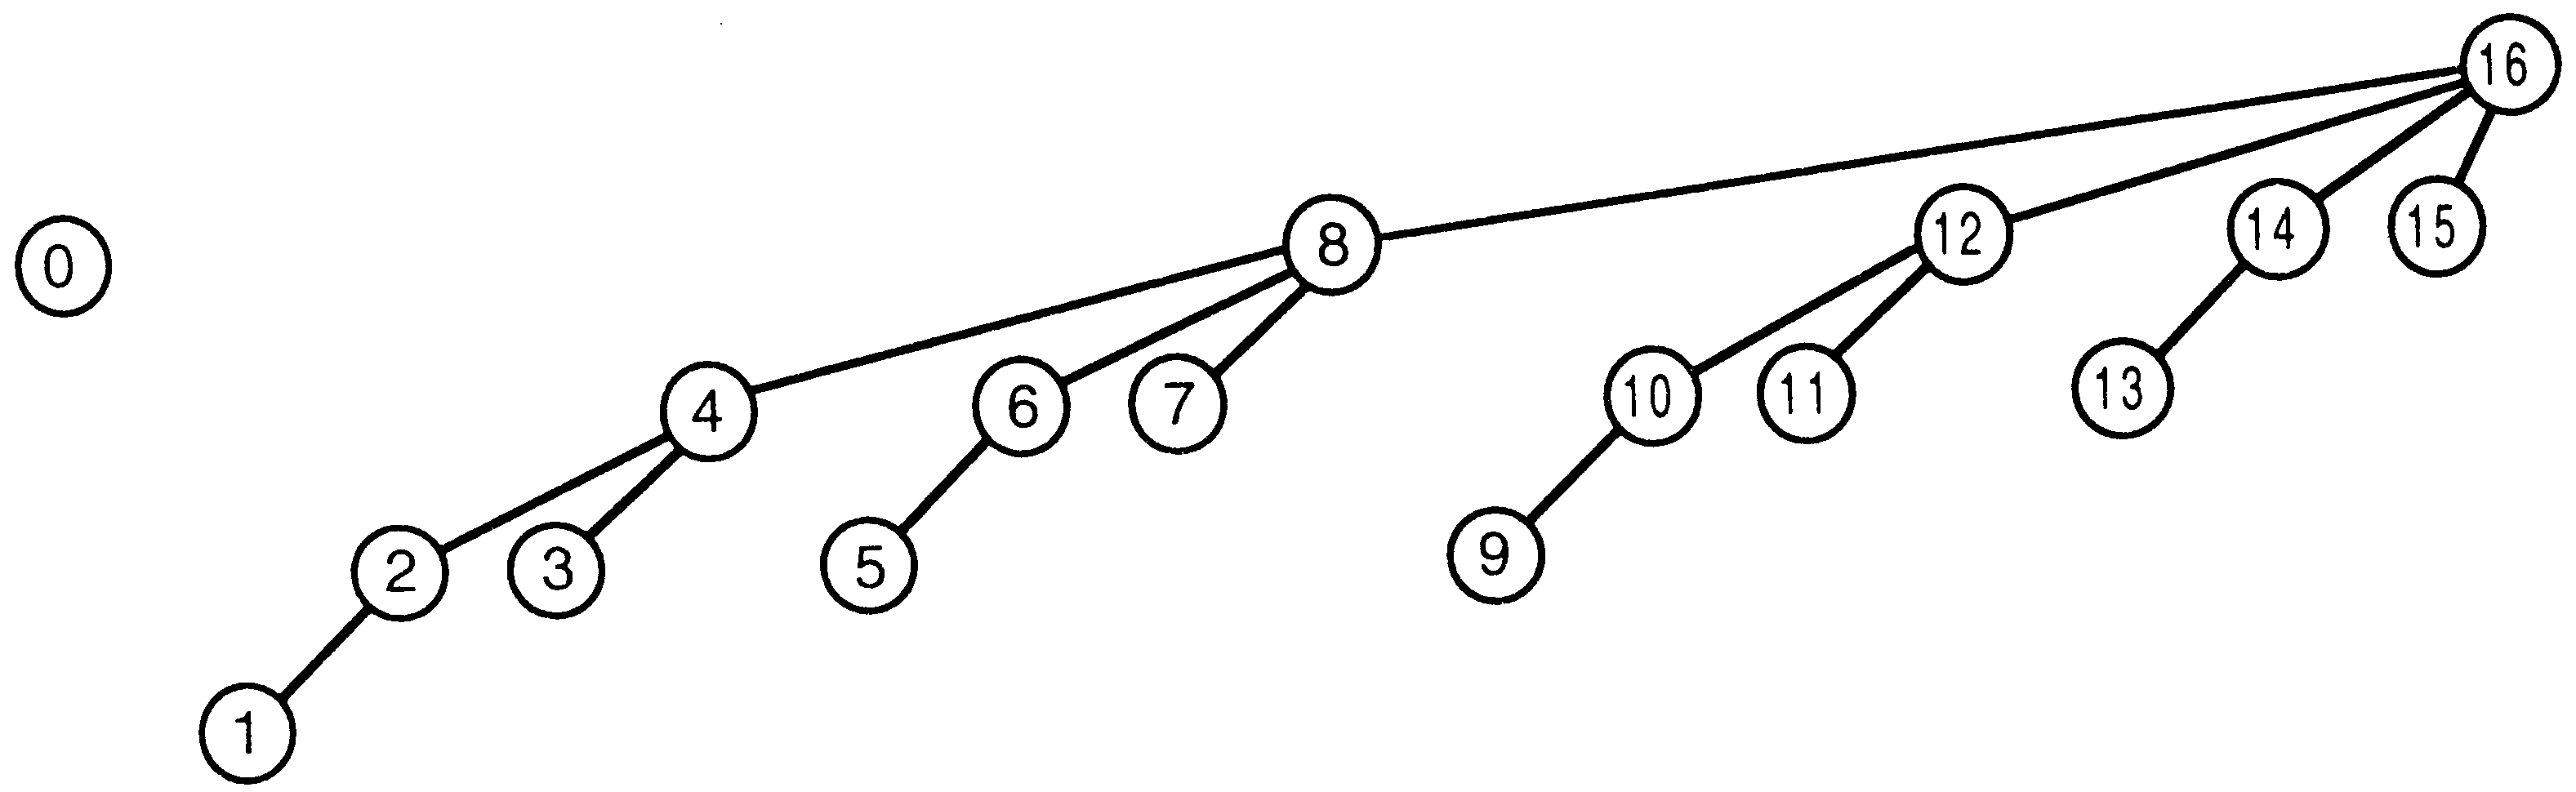
\includegraphics[height=1.7cm]{upseq.png}
				\footnote{引用自A New Data Structure for Cumulative Frequency Tables by Fenwick} 
			\end{frame}
			\begin{frame}{正确性和复杂度分析}
				然后我们可以证明如下性质:
				\begin{theorem}
					对于任意$1 \leq a \leq b \leq n$,$a$的递增序列与$b$的递减序列有且仅有一个元素相同。 
				\end{theorem}
				\begin{proof}
					如果有,则唯一是显然的,为什么有呢,如果$a$、$b$相等,则两个序列的第一个元素相等,
					如果$a$、$b$不等,假设二进制表示下$a$、$b$的最高的$k$个$1$位置相同,
					则两个序列包含$b$的前$i+1$个$1$或前$i$个$1$所代表的那个数。
				\end{proof}
			\end{frame}
			\begin{frame}{正确性和复杂度分析}
				通过上面的结论,我们考虑:\\
				若我们每次给位置$i$加$x$时,将位置$i$所对应的递增序列对应位置都加$x$,查询时只需将$r$
				的递减序列对应位置的值加起来,就得到了我们想要的前缀和。\\
				若我们想实现区间修改、单点查询,也是类似,假如我想将前$r$个数都加$x$,只需将$r$的递减序列
				对应位置加$x$,查询$i$时将$i$的递增序列加起来就是答案。
			\end{frame}
		\subsection{应用、扩展、局限}
			\begin{frame}{应用、扩展、局限}
				树状数组除了上面提到的两个应用还可以用于:
				\begin{enumerate}
					\item 套其他数据结构(因为其对空间的高效利用和简单,比线段树更适合作为最外层)
					\item 用于二分
					\item 很容易扩展到高维情况(算是第一种的特例吧)
				\end{enumerate}
				可以通过多维护一些东西实现区间修改和区间查询(但我感觉并没有比线段树简单)。\\
				应用树状数组,需要满足:
				\begin{enumerate}
					\item 下标范围从$1$开始(可调整使其满足)
					\item 满足可减性:$[l,r]$的答案可以通过$[1,l-1]$和$[1,r]$得到,比如区间最大值就不满足。
				\end{enumerate}
			\end{frame} 
	\section{线段树}
		\subsection{简介}
			\begin{frame}{什么是线段树?}
				首先,关于线段树,有以下几个要点:
				\begin{itemize}
					\item 它是一颗比较“匀称”的二叉树
					\item 树的每个节点代表了原数组的一个区间
					\item 树的叶子节点代表的区间只有一个元素
					\item 树的内部节点所代表的区间是它两个儿子按顺序拼接起来构成的
					\item 树节点数目等于$2 \cdot n - 1$
					\item 原数组的任何一个区间都可以被$log(n)$个线段树的节点表示
				\end{itemize}
			\end{frame}
			\begin{frame}{让我们看一下图}
				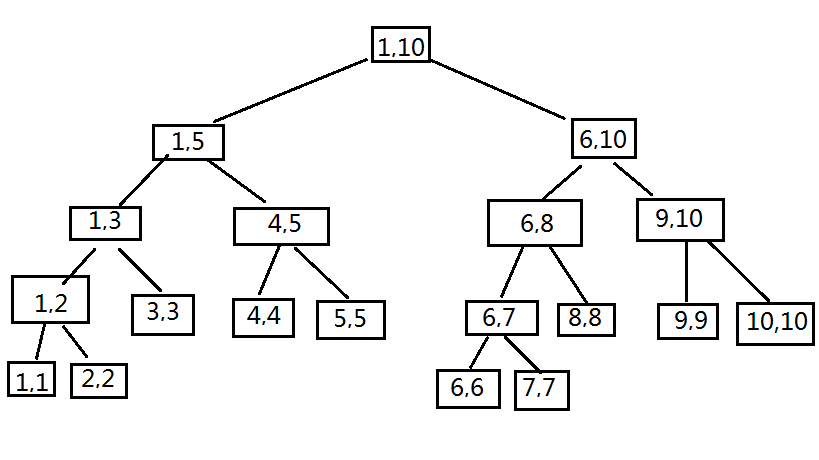
\includegraphics[height=6cm]{segtree.png}
			\end{frame}
		\subsection{能解决什么问题?}
			\begin{frame}{这种结构有什么用呢?}
				我们将这颗树建立起来,然后每个节点维护一下我们需要的关于其对应区间的信息。叶子节点的信息我们可以立即得到,内部节点的信息我们可以通过其子节点的信息合并得到。查询的时候我们只需要将查询区间对应的$log$个区间的信息合并,就得到了答案。假如我们只修改一个一个位置的值,那么只需要更新最多$log$个区间的信息。让我们来看一个最简单的例子:
				\begin{block}{单点修改,区间求最值}
					给你$n$个数:$a_1, a_2, \dots , a_n$,再给出$m$个询问:$query\;l\;r$,每次询问区间$[l,r]$的最小值和最大值,要求每个询问$O(log(n))$回答。
				\end{block} 
			\end{frame}
			\begin{frame}{如果我们需要修改区间怎么办?}
				“懒操作”!\\
				让我们再来看一个例子。
				\begin{block}{区间修改,区间求和}
					给你$n$个数:$a_1, a_2, \dots , a_n$,再给出$m$个操作,有两种操作:
					\begin{enumerate}
						\item  $modify\;l\;r\;delta$:给$[l,r]$中的每一个数加上$delta$。
						\item $query\;l\;r$:求出$[l,r]$的和。
					\end{enumerate}
					要求每个操作$O(log(n))$完成。
				\end{block}
			\end{frame}
		\subsection{总结一下}
			\begin{frame}{总结}
				我们看看线段树能解决怎样的问题。\\
				\begin{itemize}
					\item 单点修改,区间查询:\\
						\begin{enumerate}
							\item 对于长度为一的情况,能立即得到答案
							\item 信息可合并( and or max min sum gcd lcm)  
						\end{enumerate}
					\item 区间修改,区间查询:\\
						\begin{enumerate}
							\item 对于任意长度的区间,修改后的答案能立即得到。
							\item 信息可合并
							\item 懒标记 + 修改操作 = 懒标记
						\end{enumerate}
					\item 另外,如果我们在每个线段中再用一个平衡树维护一下该线段的元素,我们还可以做一些其他事情(比如找某个区间的中位数)。
				\end{itemize}
			\end{frame} 
	\section{ST表}
		\subsection{介绍}
			\begin{frame}{ST表}
				上面我们讨论的都是支持修改和查询的数据结构,我们还有一些数据结构,它们不支持修改,建立以后只支持查询操作。\\
				ST表就是其中一类,其在OI中最常用的地方是求树的lca,还可以支持快速查询某区间信息的问题(比如$O(1)$查询区间最大值)。\\
				其也很容易扩展到高维情况,从而解决一些树套树很难或不能解决的问题。
			\end{frame} 
		\subsection{例子}
			\begin{frame}{例子}
				求树的lca有点特殊,我们先以以下问题为例:\\
				\begin{block}{区间最大值}
					给你$n$个数:$a_1, a_2, \dots , a_n$,再给出$m$个询问:$query l r$,每次询问区间$[l,r]$的最大值,要求每个询问$O(1)$回答。
				\end{block} 
			\end{frame} 
		\subsection{一般化}
			\begin{frame}{其它情形呢}
				只要我们要询问的信息满足:$[a,b]$ 的信息可以由$[a,c],[d,b],  其中[a,b] = [a,c] U [d,b] $的信息得到,那么我们就可以用ST表实现$O(1)$查询(gcd lcm and or min max)。并且很容易将线性推广到高维情形。
			\end{frame} 
\end{document} 

